\documentclass{beamer}
\usepackage{graphicx}
\usepackage{caption}
%\usepackage{subcaption}
\usepackage{color}
\usepackage{amssymb}
\usepackage{xcolor}
\usepackage{wrapfig}
\usepackage{amsmath}
\usepackage[
backend=bibtex,
sorting=none,
style=authoryear
]{biblatex}
\addbibresource{bibliography.bib}

\defbibenvironment{nolabelbib}
  {\list
     {}
     {\setlength{\leftmargin}{\bibhang}%
      \setlength{\itemindent}{-\leftmargin}%
      \setlength{\itemsep}{\bibitemsep}%
      \setlength{\parsep}{\bibparsep}}}
  {\endlist}
  {\item}

\setbeamertemplate{navigation symbols}{}
\usetheme{CambridgeUS}
\usecolortheme{beaver} 

\beamersetuncovermixins{\opaqueness<1>{25}}{\opaqueness<2->{15}}

%\pgfdeclareimage[height=2cm]{i4}{pic/acat.pdf}


%\author[Dzmitry Makatun]{\textbf{Dzmitry~Makatun} \inst{1} $^{,}$ \inst{2}}

\author[Dzmitry Makatun]{\textbf{Dzmitry~Makatun} \inst{1} \inst{3} \and J\'er\^ome~Lauret\inst{2}\\ \and Michal~\v{S}umbera \inst{1} \and Hana~Rudov\'a \inst{4}}
\title[FJFI, \v{C}VUT]{Distributed Data Processing for High Energy Physics} 
\institute [KM, FJFI]
{ 
  \inst{1}%
  Nuclear Physics Institute, Academy of Sciences, Czech Republic
  \pgfdeclareimage[height=2cm]{i1}{pic/ujf.pdf}   
  \and
  \inst{2}%
  Brookhaven National Laboratory, USA
  \pgfdeclareimage[height=2cm]{i2}{pic/STAR.pdf}
  \and
  \inst{3}
Czech Technical University in Prague, Czech Republic  
\pgfdeclareimage[height=2cm]{i3}{pic/ctu.pdf} 
\and
\inst{4}
Faculty of Informatics, Masaryk University, Czech Republic
\pgfdeclareimage[height=2cm]{i6}{pic/fjfi.pdf}
\pgfdeclareimage[height=2cm]{i8}{pic/doe.pdf}
 
\vspace{-4mm}   
  \pgfuseimage{i1}
  \pgfuseimage{i2}
  \pgfuseimage{i3}
  %\pgfuseimage{i4}
  %\pgfuseimage{i5}
  %\pgfuseimage{i6}
  %\pgfuseimage{i8}

  \vspace{-7mm}
\begin{center}
d.i.makatun@gmail.com
\end{center}
\vspace{-5mm}
  }
\begin{document}
\date{\today} 

\begin{frame}
\titlepage
\end{frame}

\begin{frame}\frametitle{Outline}\tableofcontents
\end{frame}

\section{Introduction}

\begin{frame}\frametitle{Computations in HEP: what do we compute?}
\begin{figure}
\begin{center}
%\vspace{-1 cm}
\includegraphics[ height=0.4\textheight]{pic/rhic.jpg}
\hspace{0.5cm}
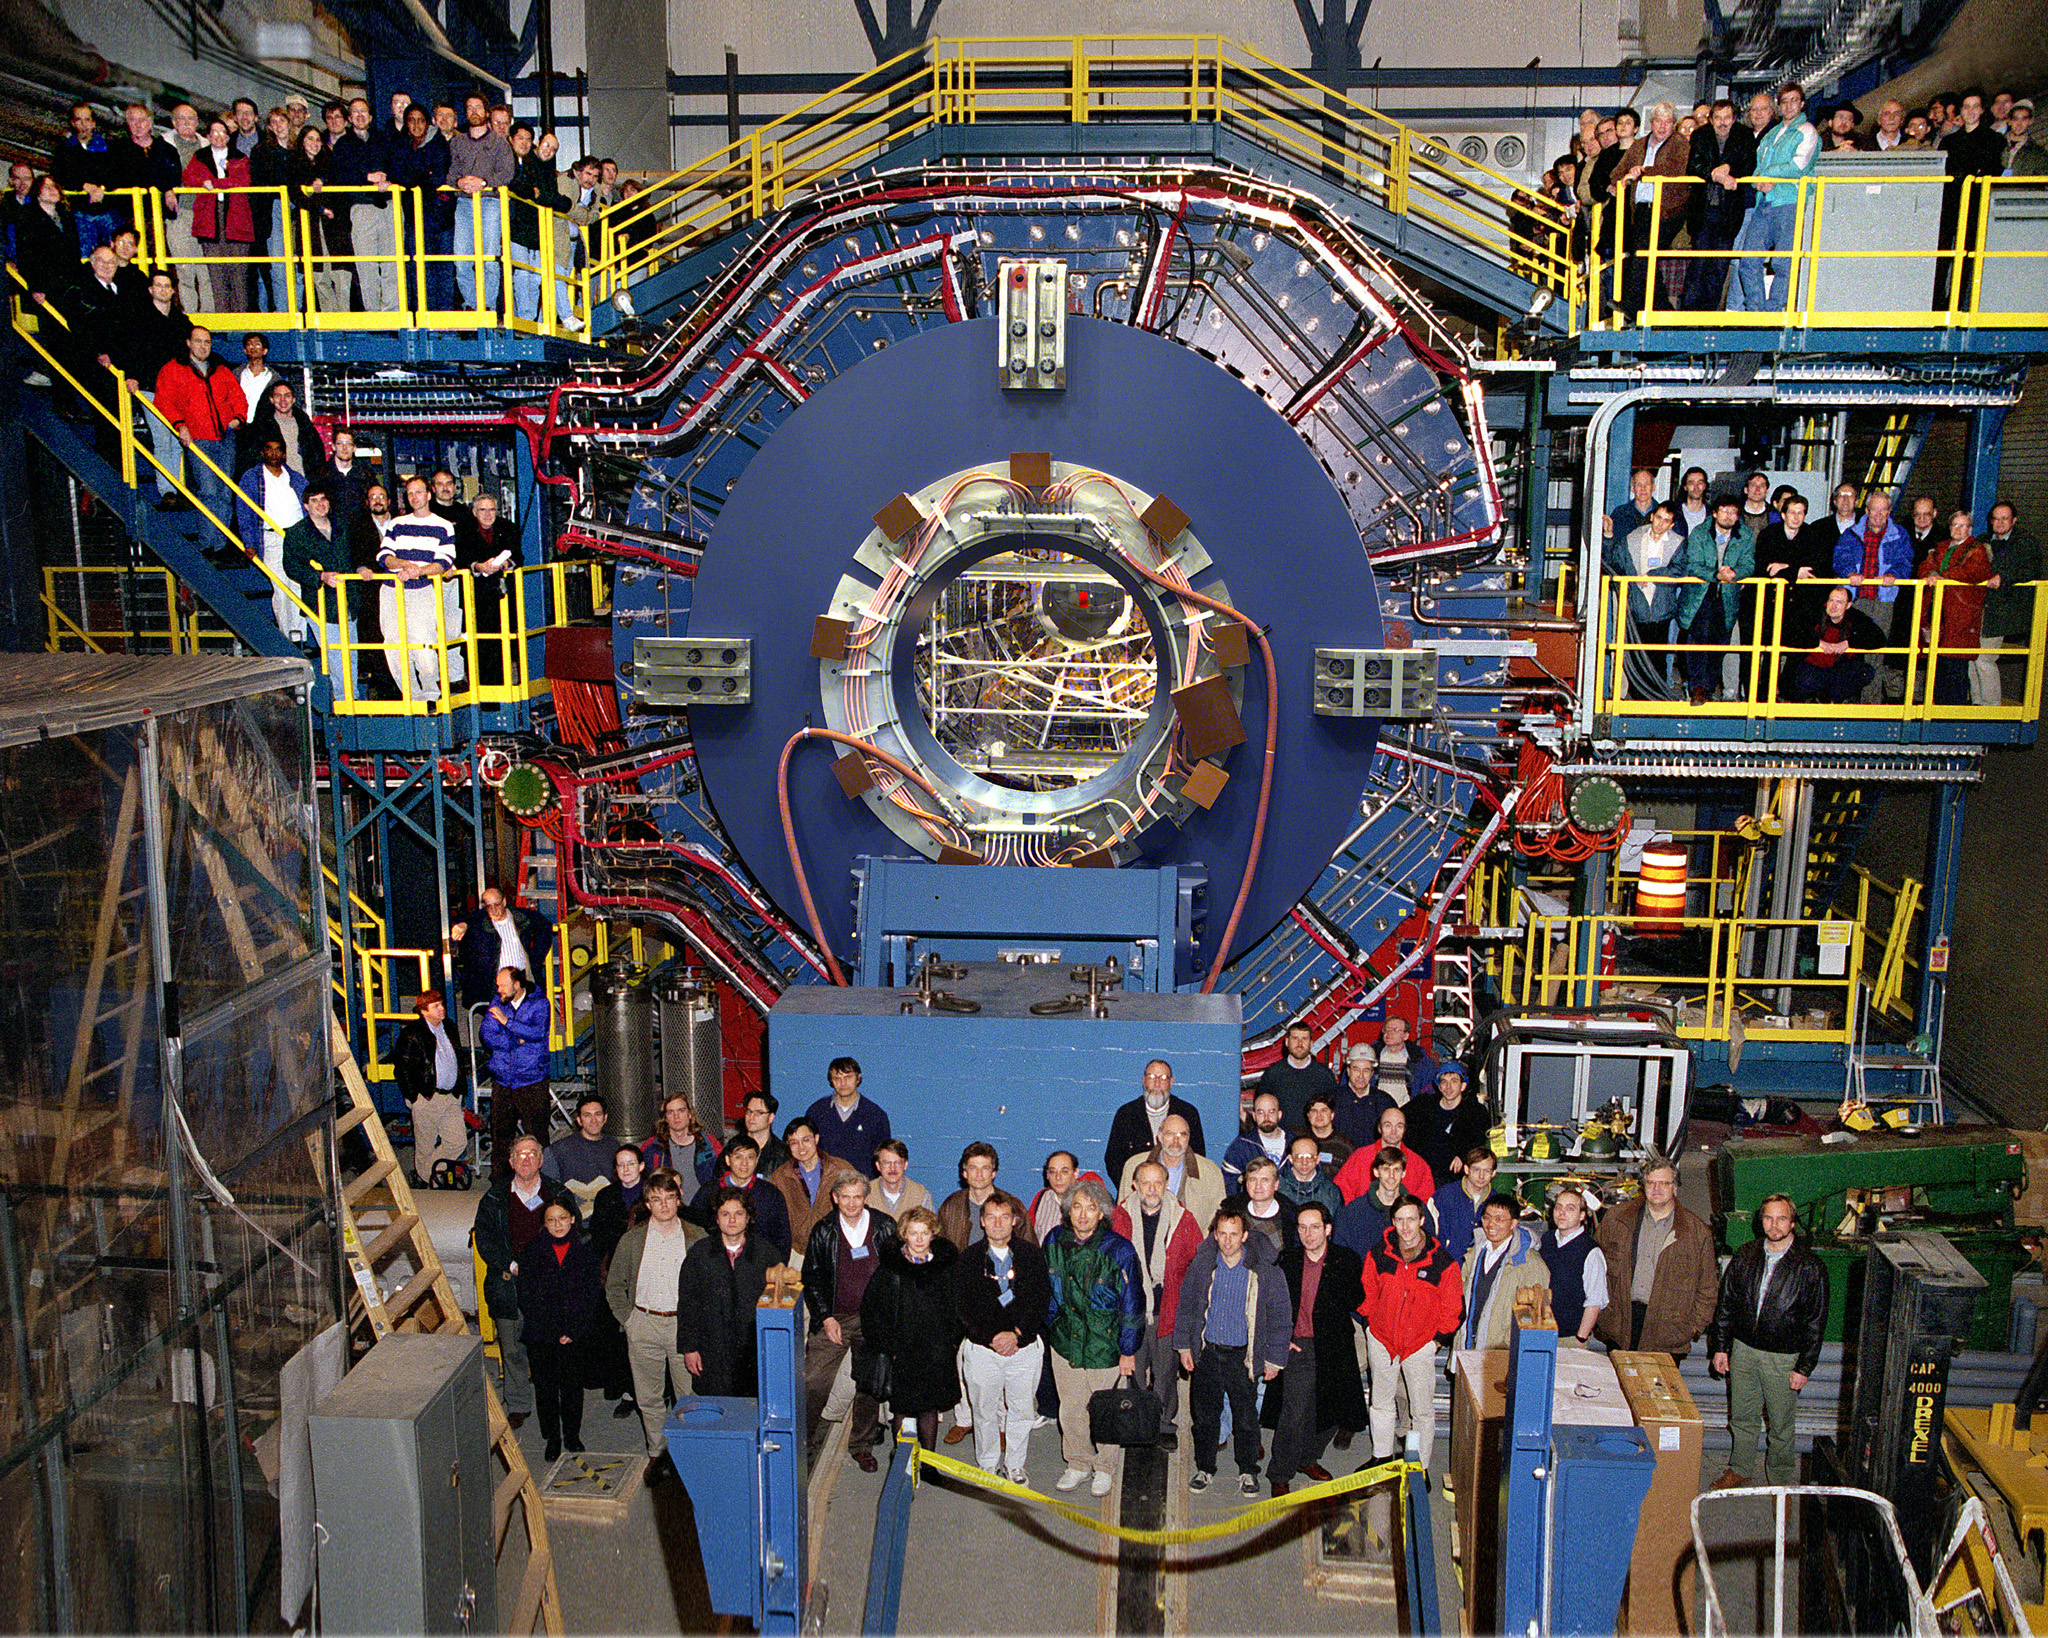
\includegraphics[ height=0.4\textheight]{pic/star.jpg}
\end{center}
\end{figure}
\vspace{-1 cm}
\begin{block}{}
		\begin{itemize}
			\item Brookhaven National Laboratory (\textbf{BNL}) Long Island, NY, USA
			\item Relativistic Heavy Ion Collider (\textbf{RHIC}). In Gold-Gold ion collisions a quark-gluon plasma is created to study the primordial form of matter that existed in the universe shortly after the Big Bang.
			\item Solenoid Tracker at RHIC (\textbf{STAR}). Collisions occur millions of times per second. Events of size 200 MB are processed at input rates up to 100Hz. Output data rate is $\sim$ \textcolor{red} {30 MB/sec}.
		\end{itemize}
 	\end{block}
\end{frame}

\begin{frame}\frametitle{Computations in HEP: how do we compute?}
\begin{block}{}
\textbf{Data Production:} The raw output data is processed to reconstruct events. ($\sim$ ones)\\
\textbf{User Analysis:} Then the reconstructed events are analyzed by scientists to discover new physics. (Each file many times)\\
All the data: raw, reconstructed and analysis output are stored.\\
31 PB of data stored on tape, $\sim$ 12 000 jobs running simultaneously (at RCF only).\\

 	\end{block}
\begin{figure}
\begin{center}
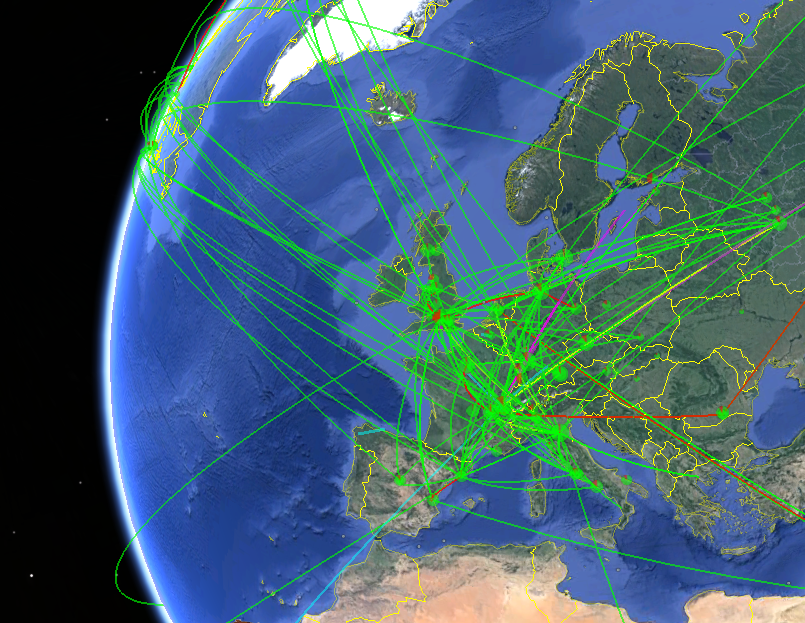
\includegraphics[ height=0.35\textheight]{pic/grid-net.png}
\hspace{0.1cm}
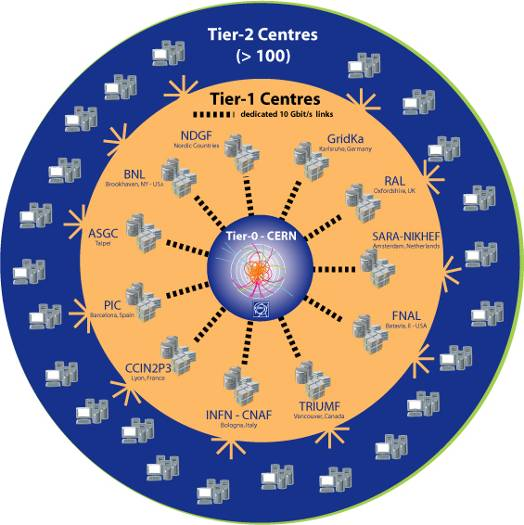
\includegraphics[ height=0.35\textheight]{pic/tiers.jpg}
\hspace{0.1cm}
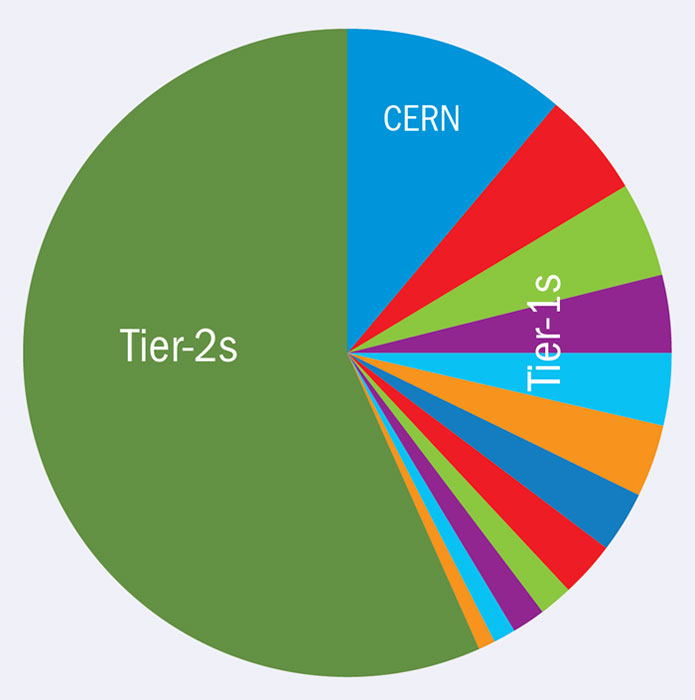
\includegraphics[ height=0.35\textheight]{pic/cern-tier-chart.jpg}
\end{center}
\end{figure} 	
\end{frame}


\subsection{Motivation}
\begin{frame}\frametitle{Motivation}
\begin{footnotesize}
\begin{block}{[\cite{Zerola}]}
Efficient and controlled movement of replicated datasets within Grid to satisfy multiple requests in the shortest time. 
 \begin{itemize}
 % add picture
\item Select between several data sources. 
\item Create optimal transfer paths, merge shared transfer paths of the same file.
\item Schedule transfers on links.
\end{itemize} 
It was shown that global planning of \textbf{data-transferring} over Grid can outperform well known heuristics (e.g. P2P, Xrootd reasoning)
\end{block}  
 		\begin{block}{\textbf{New goal: Problem extension}}
Global planning for \textbf{jobs coupled with transfers} in distributed environment.
 	\end{block} 	
\vspace{-2mm}
\begin{block}{Example of decisions} 
		\begin{itemize}
			\item[?] Send a job to a site with slow connection \textbf{or} wait for a free slot at local site?
		\item[?] Access data remotely \textbf{or} transfer it before the job starts?	
		\end{itemize}
\vspace{-2mm}		
Heuristics in use  \texttt{[Pull a job when CPU slot is free]} will not give the answer.

\end{block}  	 	
\end{footnotesize} 	
\end{frame}


\subsection{Problem analysis}
\begin{frame}\frametitle{Case 1: Data production. Planning remote site usage. }
 	\begin{columns}[c] % the "c" option specifies center vertical alignment
    \column{.6\textwidth} % column designated by a command 	
    \begin{footnotesize}
    \vspace{-11mm}
	\begin{block}{}
		\begin{itemize}
		\item RAW data is located at BNL.
		\item Computational resources are available at BNL and several remote sites.
		\item 1 job per file.
		\item 1 CPU per job. 
		\item Input size $\approx$ Output size
		\item Output file has to be transferred back to BNL.
		\item \textbf{How should we distribute a given set of files between sites to complete the processing faster?}
		\end{itemize}
 	\end{block} 	
 	
 	\begin{block}{}
 	Manually adjust the number of remote jobs to meet the network throughput, \textbf{but} what if:
		\begin{itemize}
		\item[-] More sites
		\item[-] Changing network load
		\end{itemize}
	This should be automated.
 	\end{block} 	
 	     

 	\end{footnotesize}
 	\column{.4\textwidth}
 		\vspace{-5mm}
		\begin{figure}   
				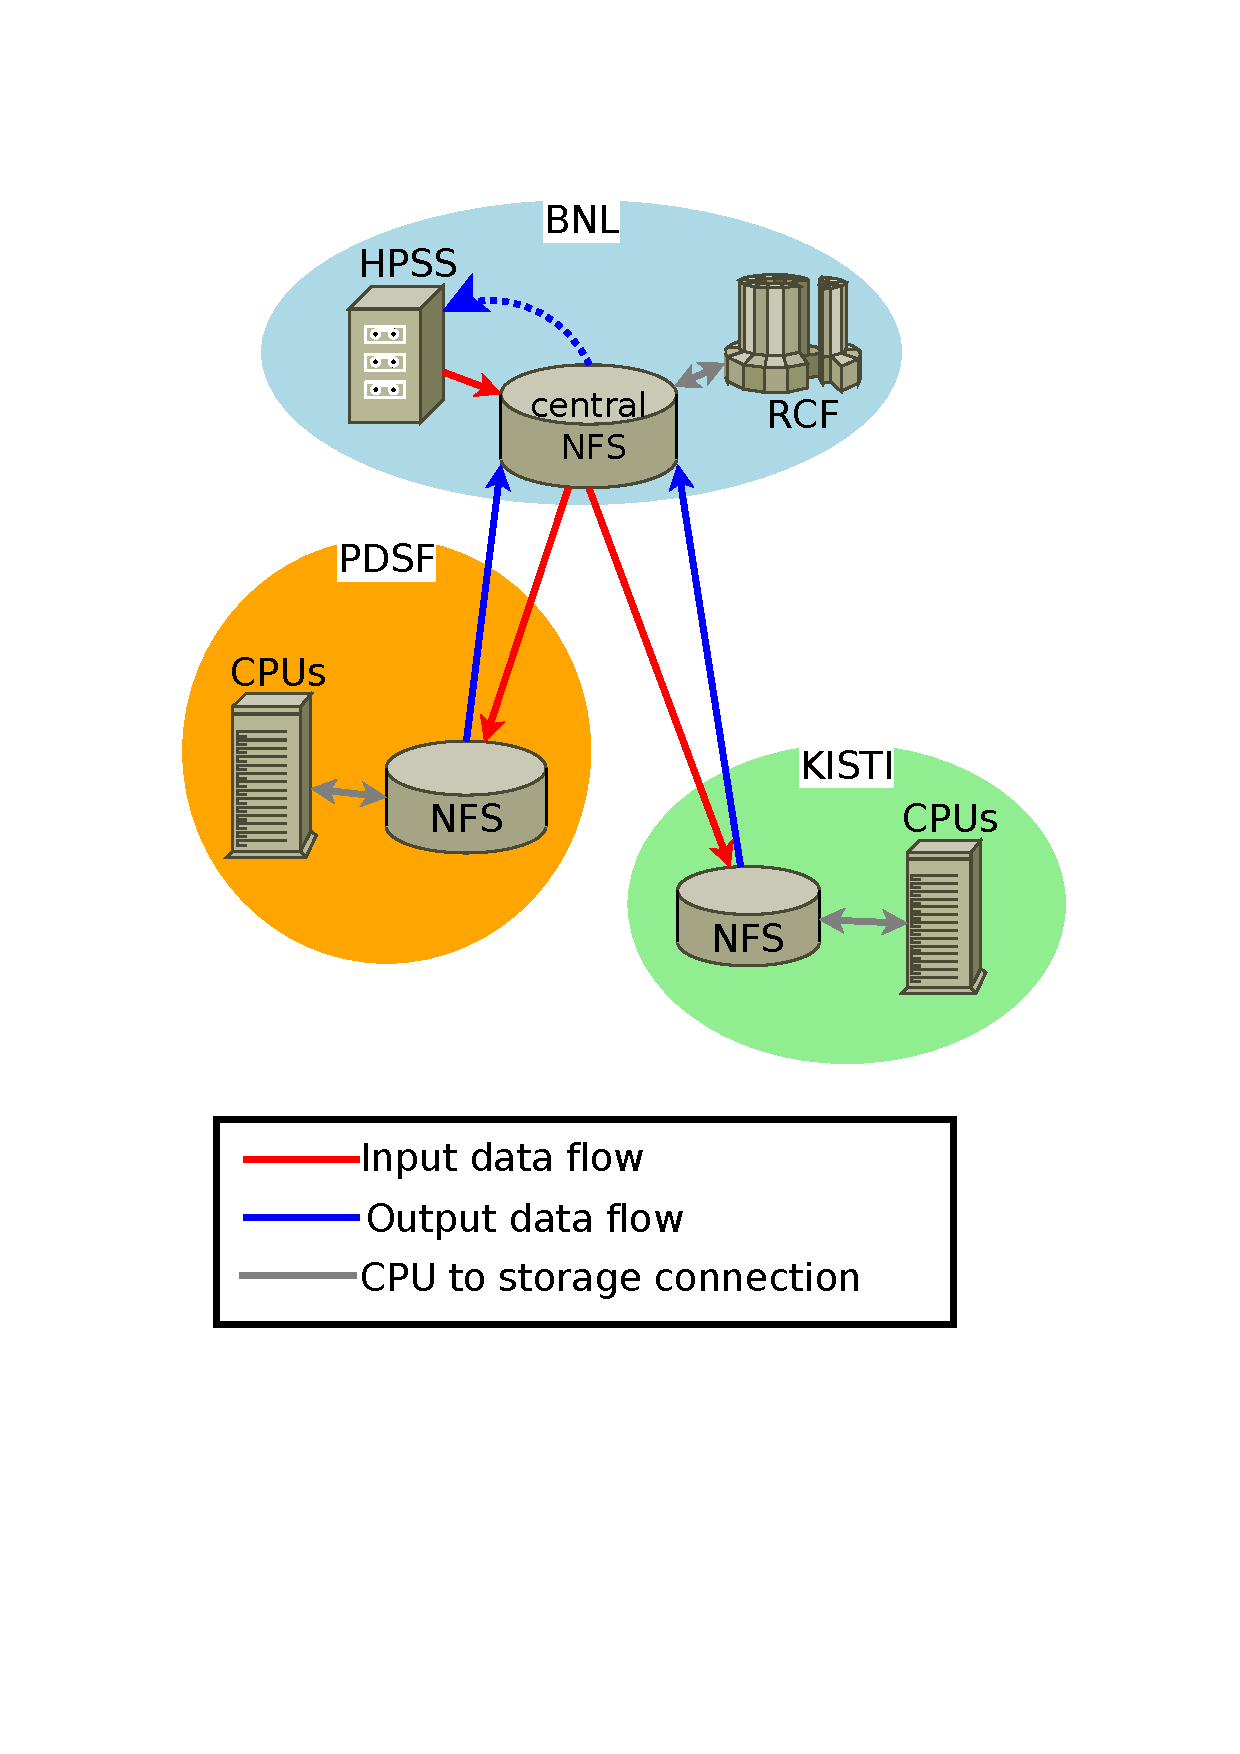
\includegraphics[trim = 25mm 10mm 0mm 30mm, clip, width=1.2\textwidth]{pic/Data_production_schema2.pdf}
		\end{figure} 	 	
 	\end{columns}
\end{frame}


\begin{frame}\frametitle{Case 2: Data production. Optimization. }
 	\begin{columns}[c] % the "c" option specifies center vertical alignment
    \column{.5\textwidth} % column designated by a command 	
    \begin{footnotesize}
    \vspace{-20mm}
	\begin{block}{New dimensions of the problem}	
		\begin{itemize}		
			\item Several possible data sources.
			\item Real network topology: shared links, links between remote sites.
			\item Limited storage at sites.
			\item \textbf{Which file source to select?}
			\item \textbf{What is the optimal transfer path?}

		\end{itemize}
 	\end{block}
		\begin{block}{Example: data-production at ANL  [\cite{Balewski}]}	
		\begin{itemize}
			\item ANL: many CPU's, but slow connection and small disk space.
			\item NERSC: fast connection, large disk.
			\item Optimization: Feed ANL from both BNL and NERCS sites.		

		\end{itemize}
 	\end{block}
 	\end{footnotesize} 
 	\column{.45\textwidth}
		\begin{figure}
			\begin{center}
			    \vspace{-15mm}
				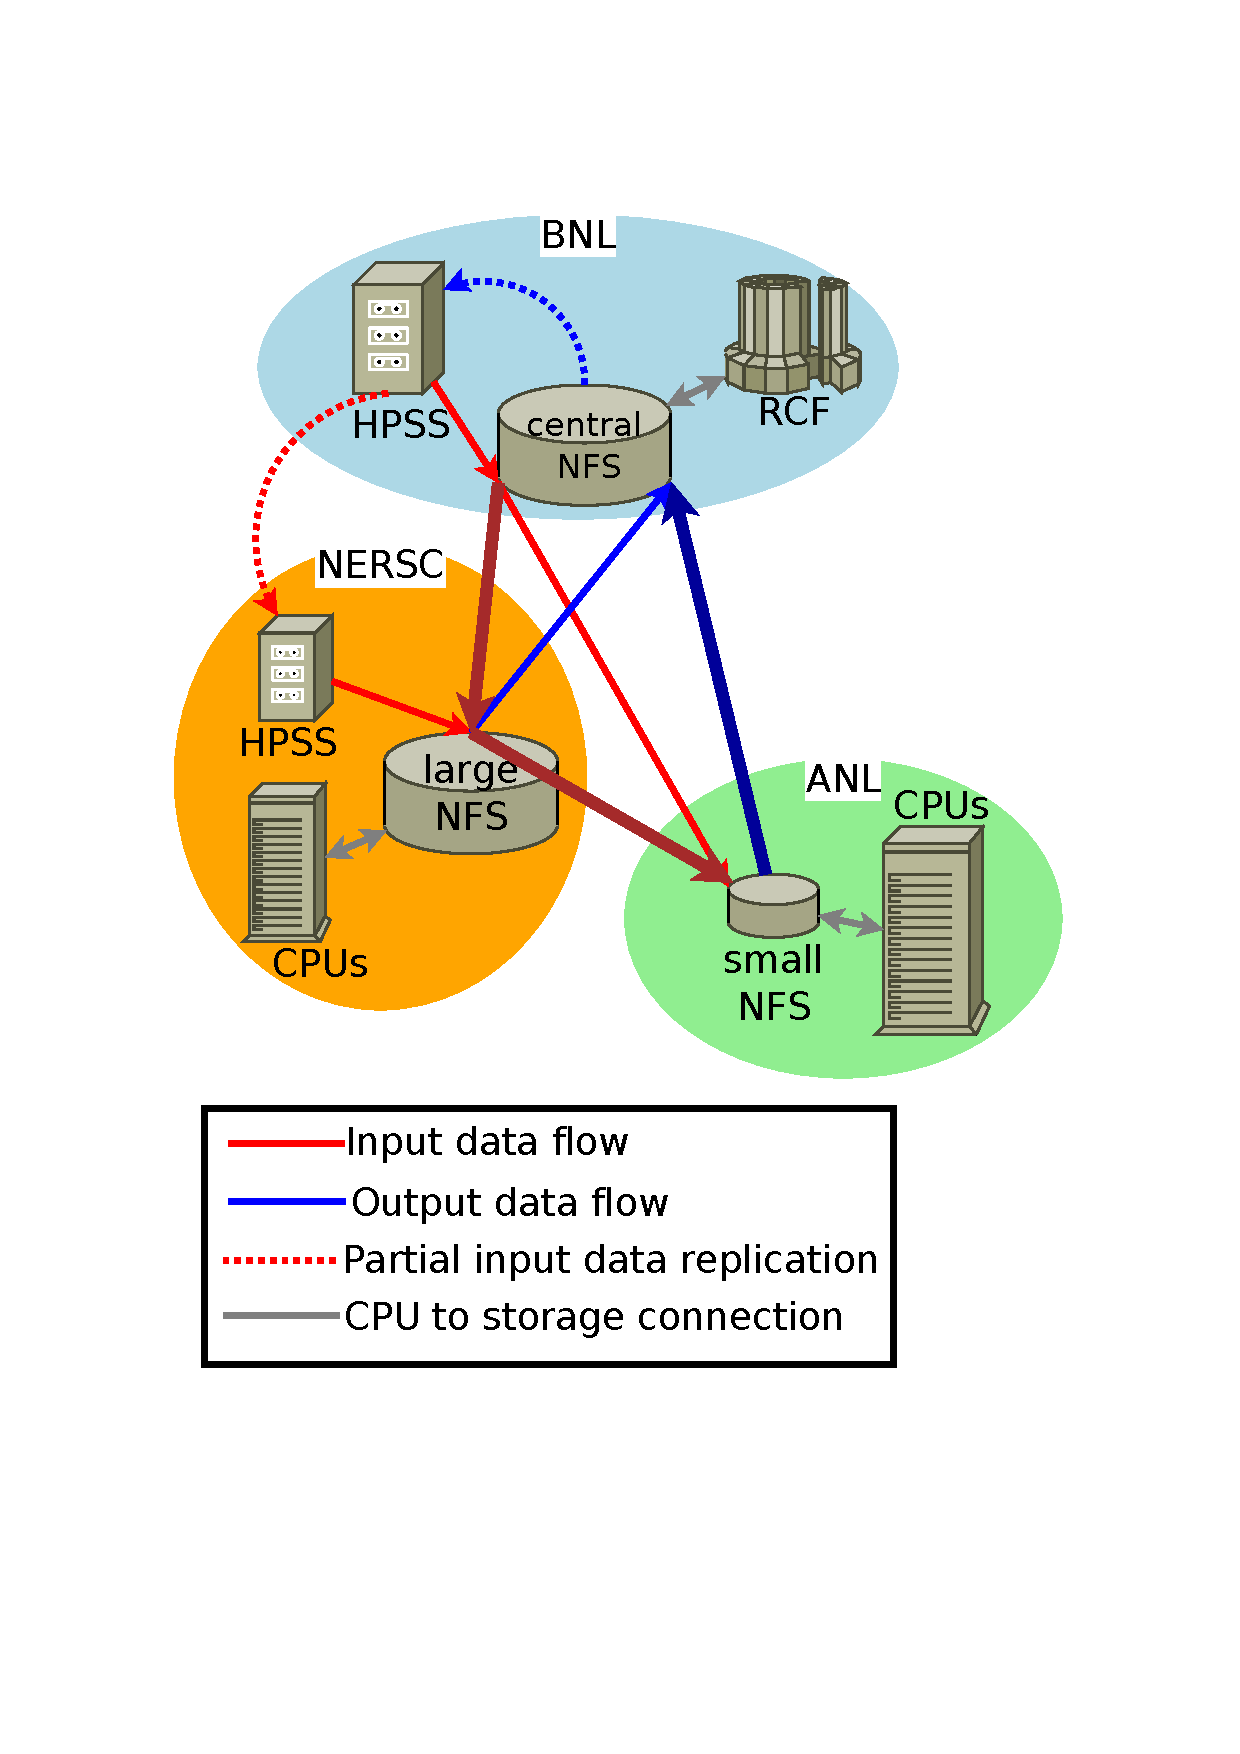
\includegraphics [width=1.2\textwidth]{pic/Data_production_schema_ANL2.pdf}
			\end{center}
			\end{figure} 	 	
 	\end{columns}
\end{frame}


\begin{frame}\frametitle{Case 3: User analysis. }
 	\begin{columns}[c] % the "c" option specifies center vertical alignment
    \column{.5\textwidth} % column designated by a command
 	\begin{small}
 	\vspace{-10mm}
	\begin{block}{New dimensions of the problem}
		\begin{itemize}
			\item Many copies of files exist.	
			\item Each file can be requested by multiple jobs.
			\item The size of output of analysis is negligible compared to input size.
			\item The processing time estimates  are imprecise.
			\item \textbf{When and where to replicate the data?}
		\end{itemize}
 	\end{block} 	
 	\end{small}
 	\column{.45\textwidth}

		\begin{figure}
			\begin{center}
			    \vspace{-15mm}
				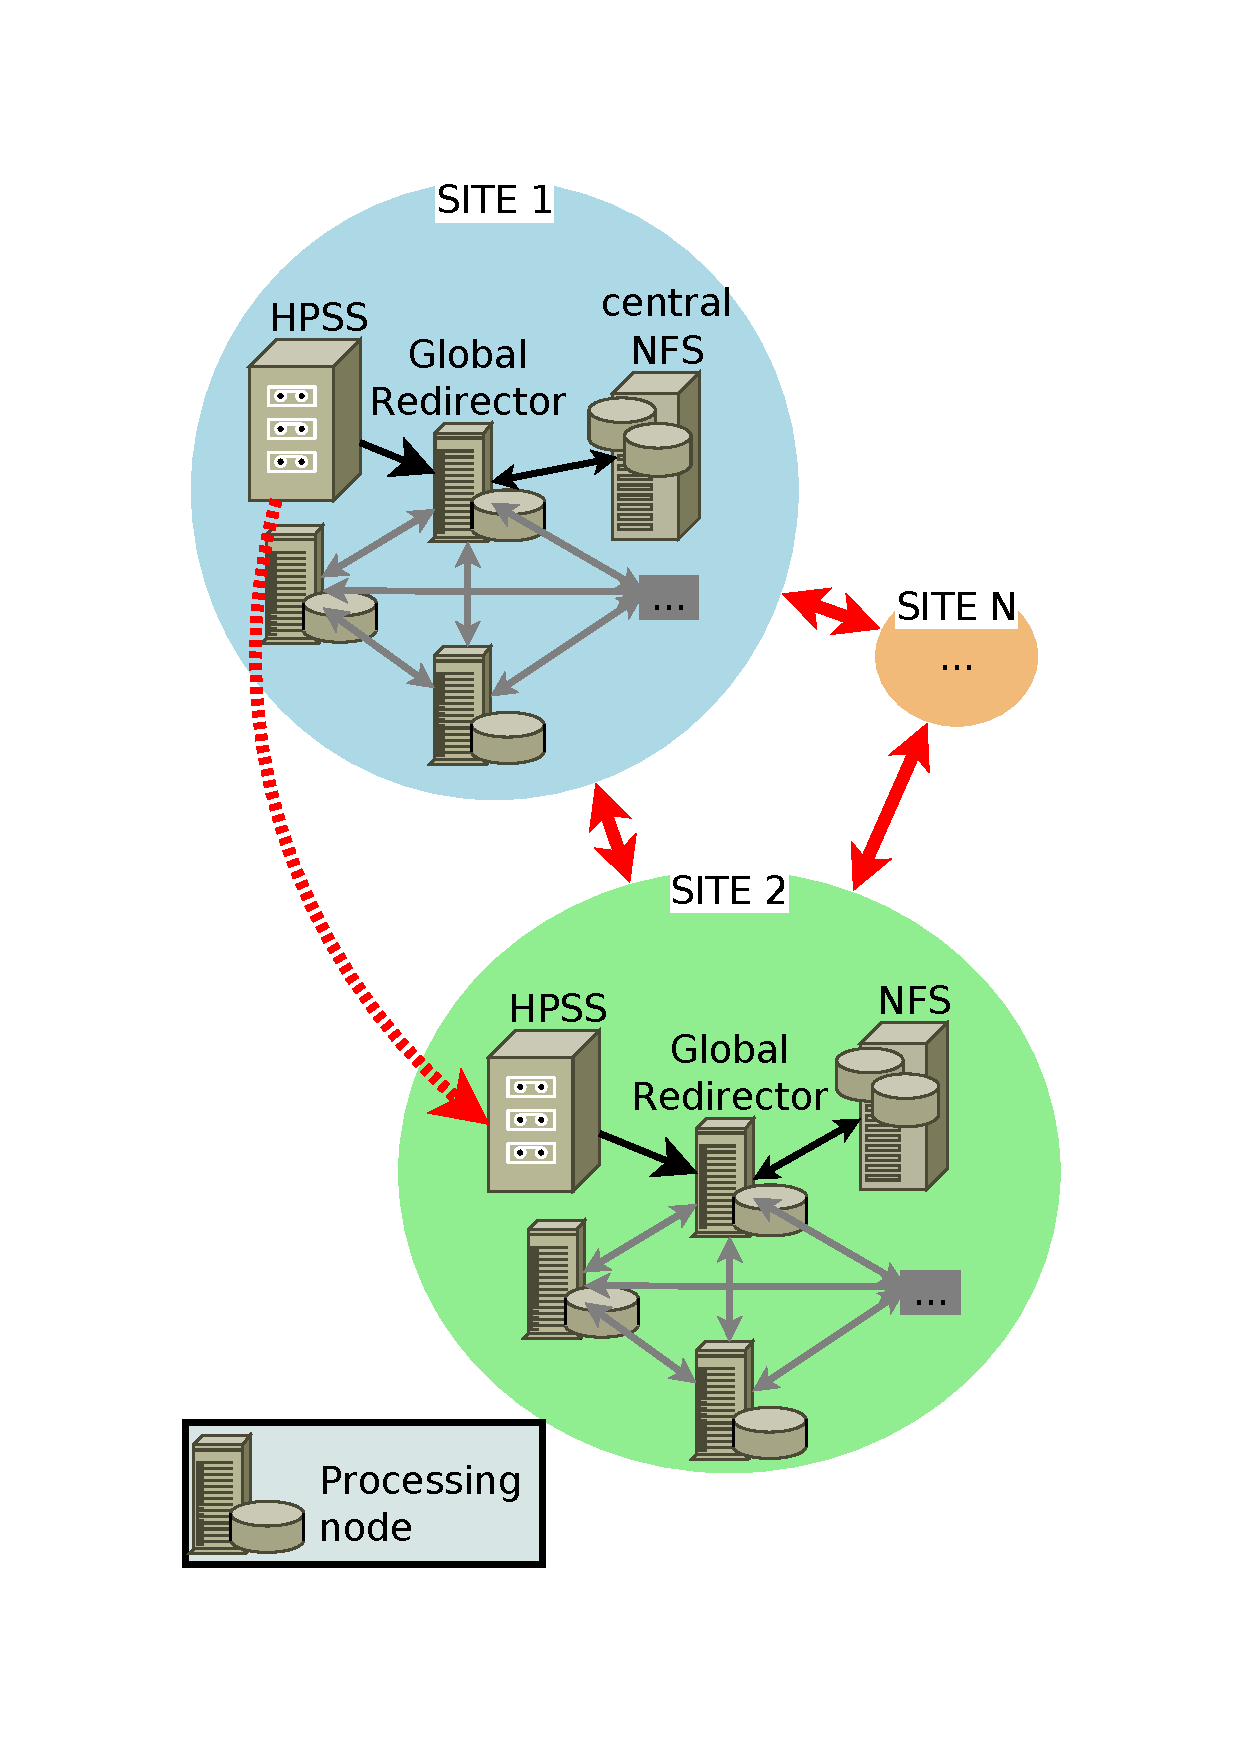
\includegraphics[ width=1.15\textwidth]{pic/user_analysis.pdf}
			\end{center}
			\end{figure} 	 	
 
 	\end{columns}
\end{frame}

\subsection{Existing solutions}
\begin{frame}\frametitle{STAR: setup for data production at a remote site (KISTI)}
\begin{figure}
\begin{center}
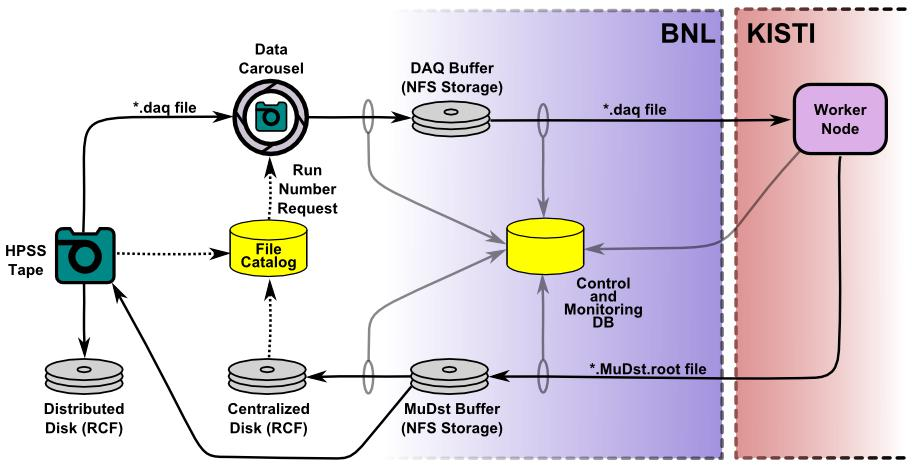
\includegraphics[ width=\textwidth]{pic/kisti_production.jpg}
\end{center}
\end{figure}
\begin{block}{}
		\begin{itemize}
			\item For better efficiency an ad-hock setup is used. \cite{KISTI}
		\end{itemize}
 	\end{block}
\end{frame}

\begin{frame}\frametitle{Existing solutions (used in HENP)} 	
\begin{block}{Batch System + Distributed Data Management System (Independent)}  
		\begin{itemize}
			\item PBS, Condor. [Pull a job from global queue]
			\item Xrootd, DPM. [Site which replies first is selected as a source] 			
		\end{itemize}
 	\end{block} 	
\begin{block}{Data Trains (For user analysis)}	
	 \begin{itemize}
	 \item Group jobs by input data $\longrightarrow$ preplace data $\longrightarrow$ start jobs simultaneously $\longrightarrow$ kill latest x\% of jobs. 
	 \item Train runs periodically. ($\sim$ ones per day)  
 	 \item Controlled by train operators. 
 	  \end{itemize}
\end{block}
\begin{block}{Globus (Decoupling jobs and transfers)} 	
\begin{itemize}
 	 \item Sends jobs to data.  
 	 \item Replicate most "popular" files. Relies on usage history.
 	 \item Where to replicate? When to replicate? No transfer planning.
 	 \end{itemize}
\end{block} 	 
\end{frame}



\begin{frame}\frametitle{Related work (not in use in HENP)} 	
\begin{footnotesize}
\begin{block}{Bandwidth-Centric Allocation of Independent Tasks on Heterogeneous Platforms [\cite{Trees}]}  
		\begin{itemize}
			\item Exact solution for maximum steady-state throughput. 
			\item Grid network is modeled as a tree (no alternative paths). Single source/destination. Input path $=$ Output path. Equal size of jobs/files.		
		\end{itemize}
 	\end{block}

\begin{block}{XSufferage [\cite{casanova2000heuristics}]
}	
\begin{itemize}
 	 \item Considers I/O transfer latency. Assigns jobs to hosts based on $Sufferage = SecondBestEstimatedMakespan - BestEstimatedMakespan$
 	 \item No path/source selection or transfer planning. Simplified network model. No storage model.
 	 \end{itemize}
\end{block}  	
 	
 	
\begin{block}{Storage Affinity [\cite{santos2005exploiting}]}	
	 \begin{itemize}
	 \item XSufferage + job replication: Executes copies of the same job at several clusters concurrently.
	 \item Simplified network model. CPU waste $\sim 25-60$\%.
 	  \end{itemize}
\end{block}

	 
\end{footnotesize}
\end{frame}




\begin{frame}\frametitle{Distributed resource management system. Architecture (Globus example) [\cite{Globus_scheduler}]}
\begin{block}{}
		\begin{itemize}
			\item  The resource broker is acting as a middle tier 
between a user and the resources by doing resource 
matching and job submission for the user. 

		\end{itemize}
 	\end{block}
 	\begin{figure}
\begin{center}
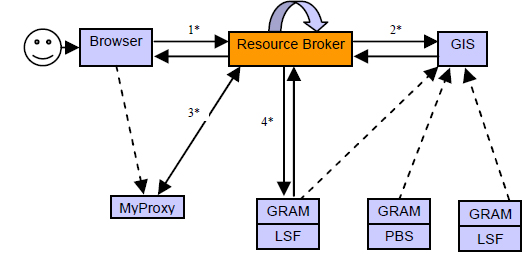
\includegraphics[ width=0.8\textwidth]{pic/resource-broker.jpg}
\end{center}
\end{figure} 	
\end{frame}

\section{Constraint Programming approach}
\subsection{Model}
\begin{frame}\frametitle{Data production problem}
 		\begin{block}{}
Create a global scheduler for Grid which will reason about:\\
\hspace{1cm} 1.data~transferring, \hspace{1cm} 2.~CPU~allocation,\hspace{1cm} 3.~data~storage.  
\end{block}
\begin{block}{Optimization}  
		\begin{itemize}
			\item None of the resources (network links, data storages and CPUs) are over-saturated at any moment of time.
			\item The jobs are executed  where the data is pre-placed.
			\item No excessive transfers or data replication.
			\item Minimal overall makespan for a given set of tasks.
		\end{itemize}
 	\end{block}
\begin{block}{}
\textbf{To solve the problem we applied Constraint programming due to its techniques for scheduling, planning and optimization.}
 	\end{block} 	
\end{frame}

\begin{frame}\frametitle{Data-production problem: Input.}
\vspace{-1cm}
\begin{center}
 	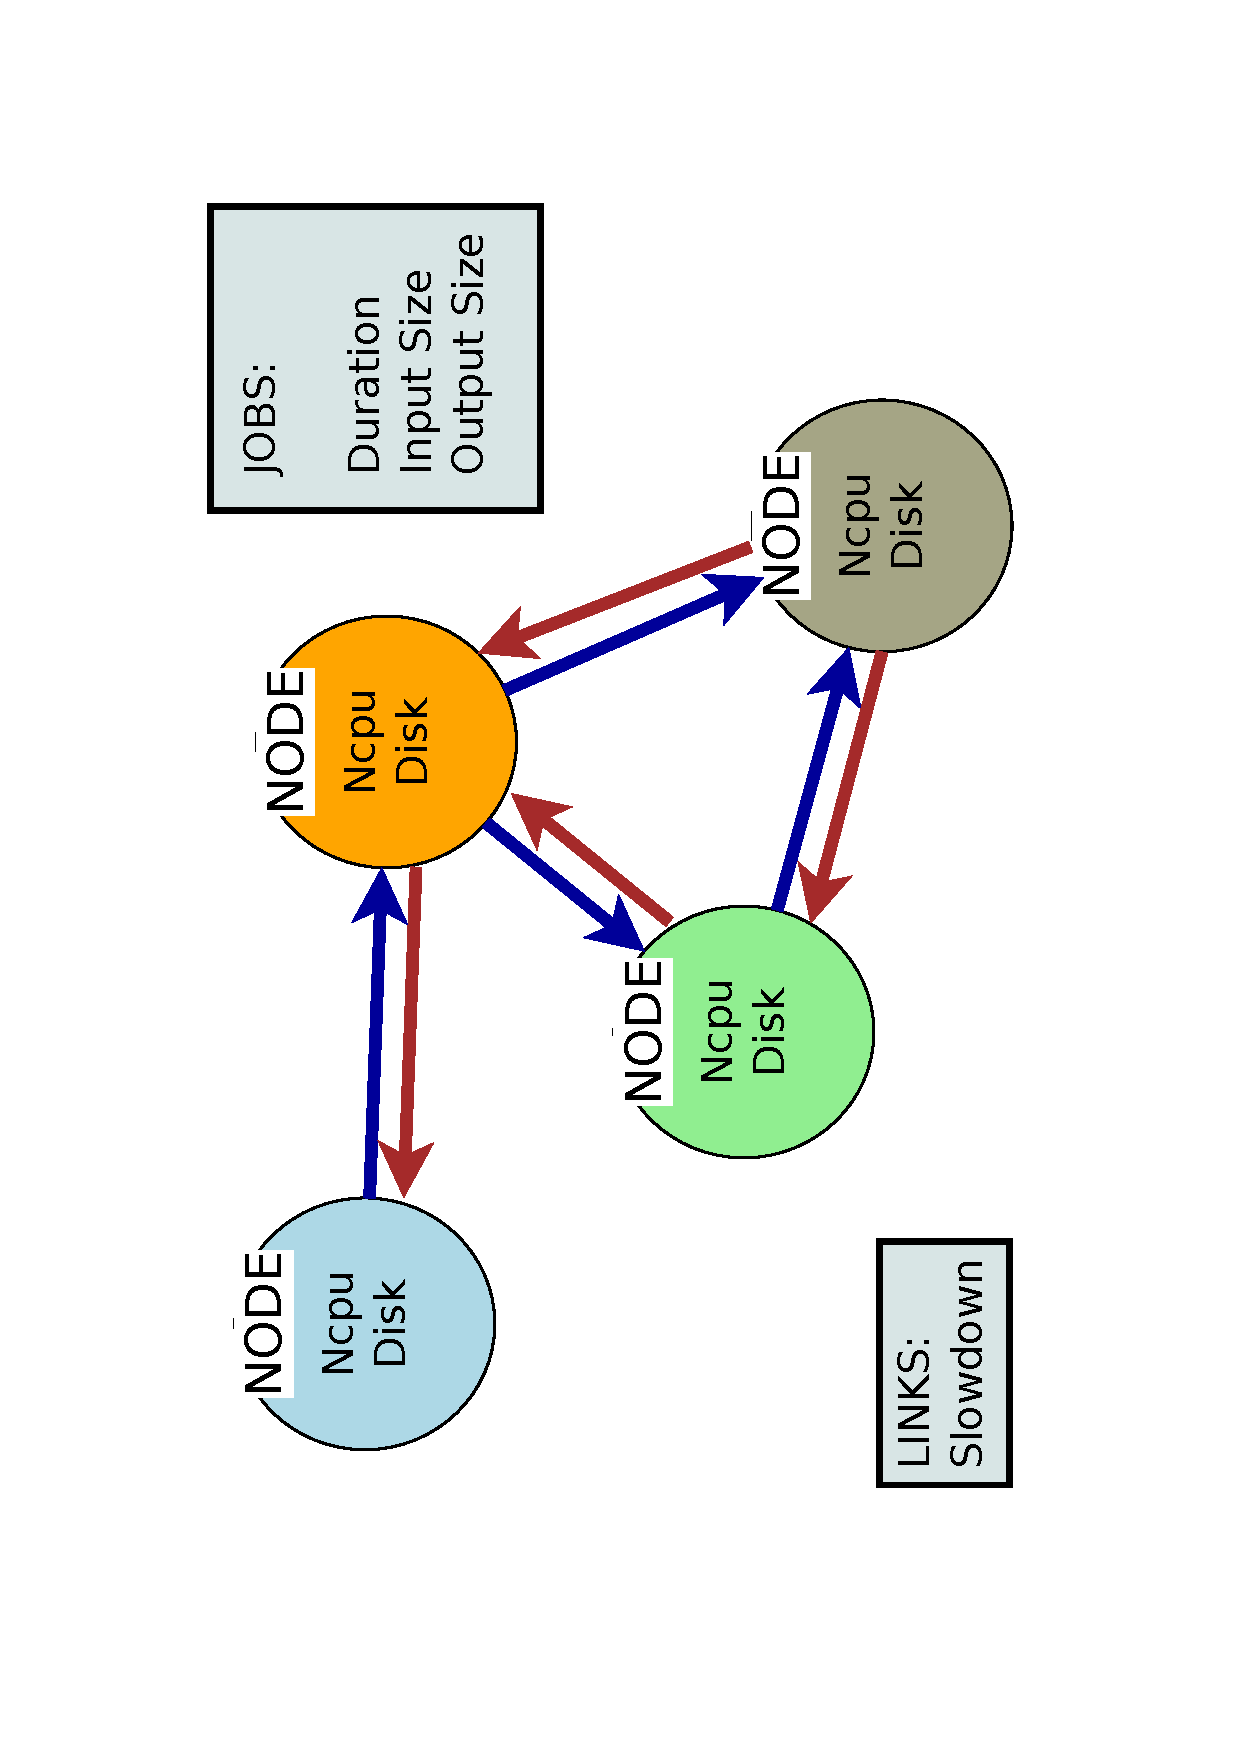
\includegraphics[trim= 30mm 0mm 10mm 0mm,clip,angle =-90, width=0.7\textwidth]{pic/network.pdf}
\end{center}
\vspace{-12mm}
\begin{block}{Assumptions}
In previous work [\cite{Zerola}] it was proved that:
		\begin{itemize}
			\item There is advantage to plan and schedule jobs by chunks (split the whole set by portions). 
					\begin{itemize}
					\item[+]More adaptability to changing environment.
					\item[+]Faster plan creation.
					\end{itemize}				
			\item The network links can be considered as unary resources: one file-transfer at a time over link.
		\end{itemize}
 	\end{block}
\end{frame}

\begin{frame}\frametitle{Solving procedure overview.}

\begin{enumerate}
\item \textbf{Initialization Stage}. Estimate $TimeLimit$.
\item \textbf{Planning Stage}. Instantiate a part of domain variables with the help of simplified constraints.     
	\begin{enumerate}[a.]
	\item Assign jobs to computational nodes. 
	\item Select transfer paths for input and output files. 
	\item Additional constraints: load balance, etc.
	\item Find a solution for the sub-problem.
	\end{enumerate}
\item \textbf{Scheduling stage}: define start time for each operation. 
	\begin{enumerate} [a.]
	\item Constraints on order of operations. 
	\item Cumulative constraints.
	\item Minimize target function: (e.g. makespan).
	\end{enumerate}
\end{enumerate}
\end{frame}


\subsection{Testing simulations}
\begin{frame}\frametitle{Simulations based on log data: problem setup.}
\begin{columns}[c] % the "c" option specifies center vertical alignment
    \column{.6\textwidth} % column designated by a command 	
    \begin{small}
\vspace{-5mm}
 		\begin{block}{Input for simulations}
		\begin{itemize}
			\item Parameters of 2000 jobs taken from log files of data production for STAR at KISTI.
			\item Jobs scheduled by chunks of 200.
			\item Slowdown of the link to the remote site proportional to the \textbf{slowdown factor}.
			\item Makespan compared to local processing.
		\end{itemize}
 	\end{block}
 		\begin{block}{Tested algorithms}
		\begin{itemize}
			\item Equal CPU load.\\ Processed by input order.
			\item Data transferred by job. \\ Processed by input order.
			\item Optimized.\\ Planner: minimize estimated makespan. Scheduler: minimize makespan.
		\end{itemize}
 	\end{block}
 	\end{small} 
 	\column{.4\textwidth}

		\begin{figure}
			\begin{center}
			    \vspace{-20mm}
				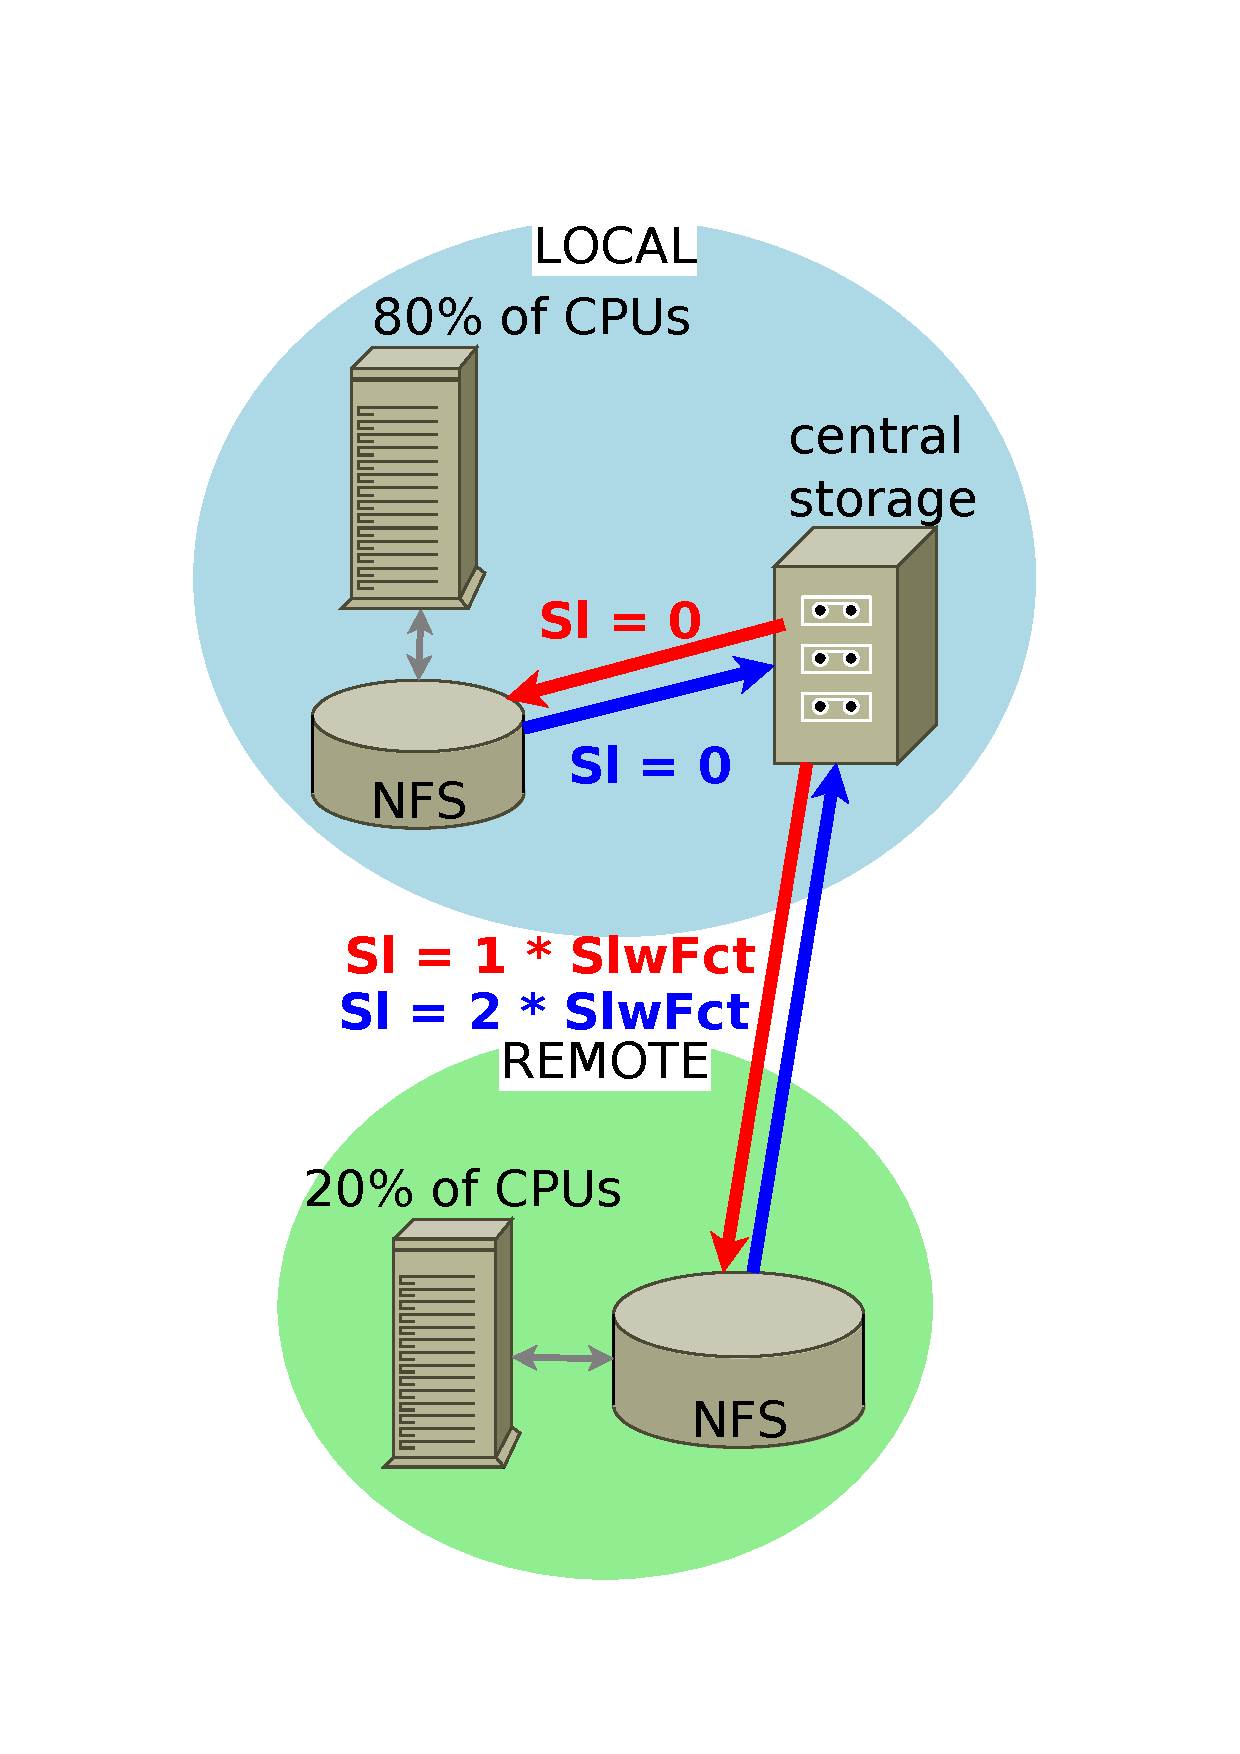
\includegraphics [width=1.2\textwidth]{pic/test_environment2.pdf}
			\end{center}
			\end{figure} 	 
\vspace{-1cm}
\begin{tiny}
\begin{center}
Constraints for storage capacity are omitted.
\end{center}
\end{tiny}
 	\end{columns} 	
\end{frame}

\begin{frame}\frametitle{Simulations based on log data: results.}
	%\vspace{-1cm}
	\begin{center}
    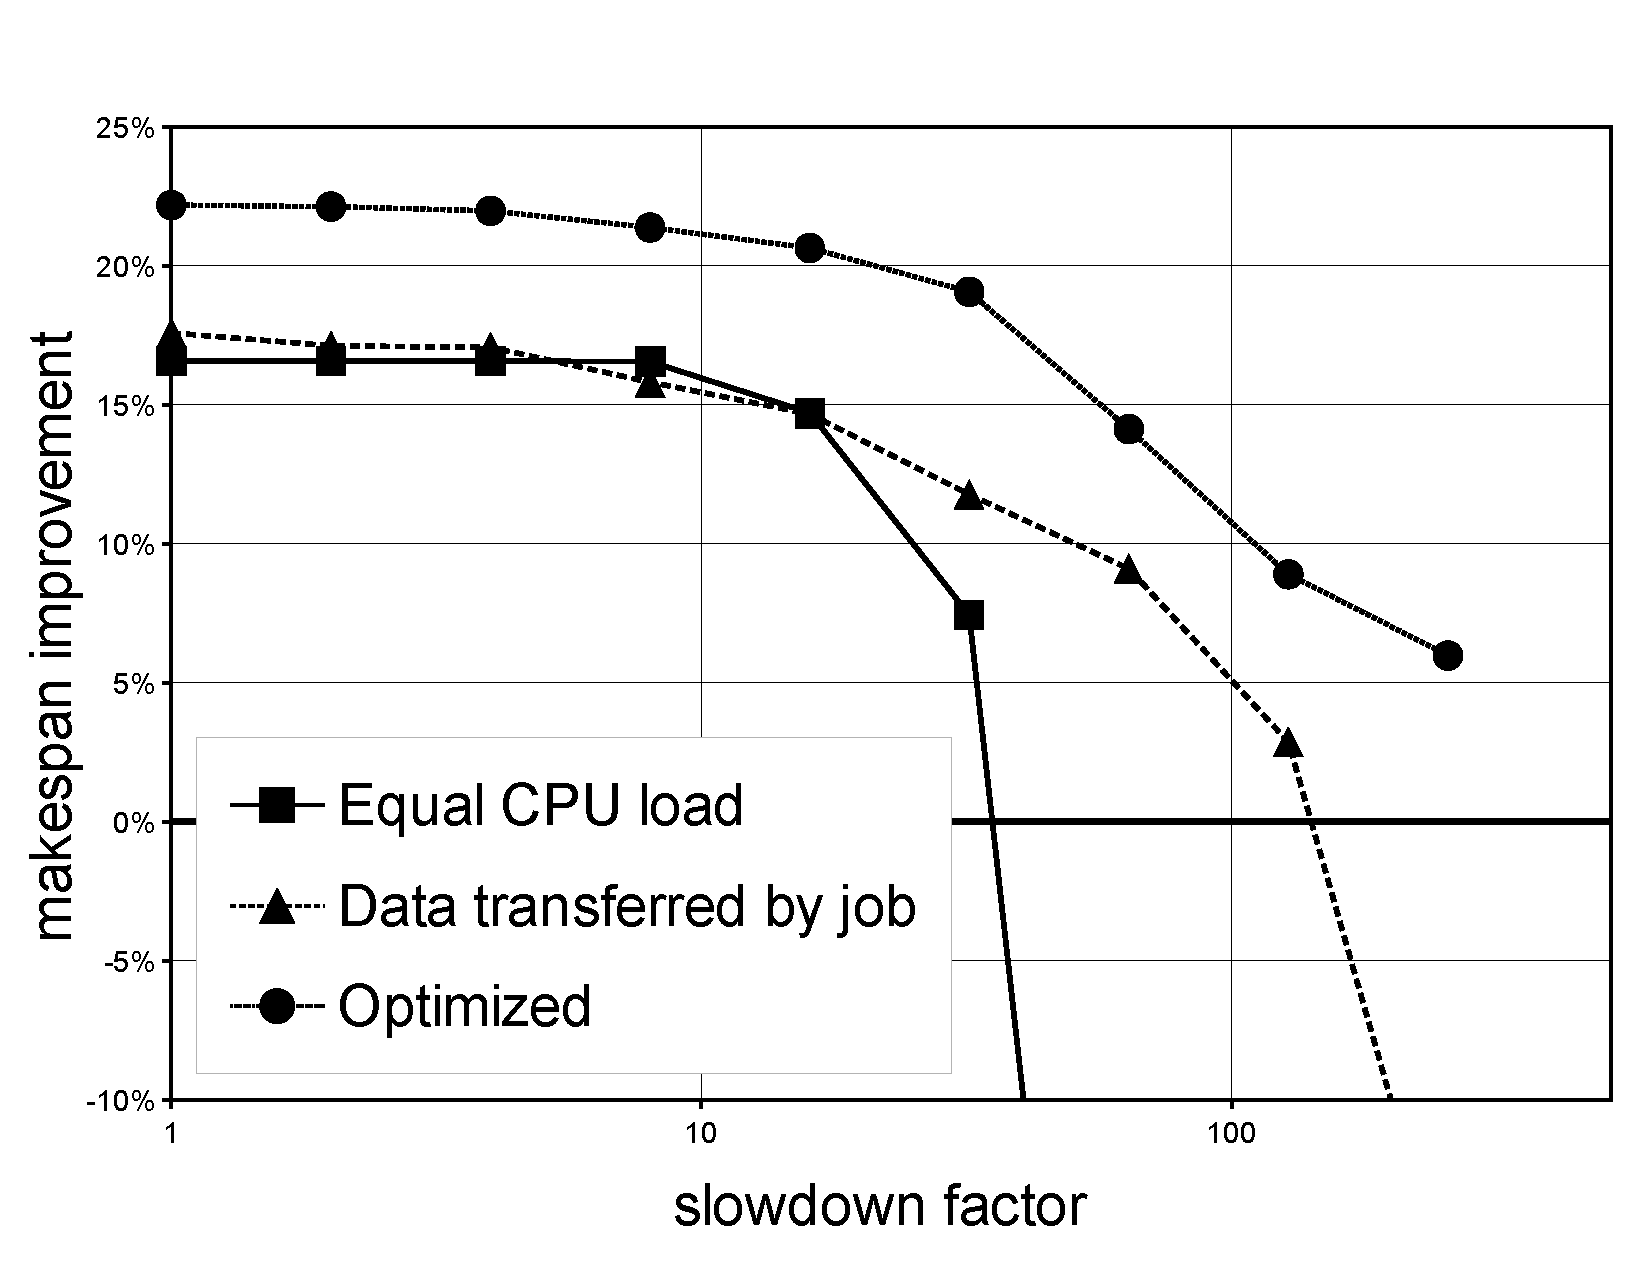
\includegraphics[trim =5mm 5mm 5mm 10mm ,clip,width=0.8\textwidth]{pic/makespan_vs_slowdown4.pdf}
	\end{center}
\end{frame}

 	
\begin{frame}\frametitle{Results of simulations}

\begin{footnotesize}
		\begin{itemize}
			\item In simulated environment, where a remote site has the same CPU number as a local site, but data transfer overhead is comparable to job duration: 
			\begin{itemize}
			\item Maintaining \textbf{equal CPU load} at local and remote sites increases the makespan more then twice; 
			\item Scheduling with \textbf{consideration of transfer overhead} can reduce makespan by 15\%.			\end{itemize}
			compared to \textbf{local only} processing.
			\item The simulations based on log files has shown that the proposed approach systematically provides a smaller makespan and adapts to the increase of transfer overheads better then the other simulated  heuristics.
			\item Proposed approach can provide \textbf{optimization} and \textbf{automatic adaptation} to fluctuating resources with no need for manual adjustment of work-flow at each site or tuning of heuristics.
		\end{itemize}		
\end{footnotesize}
\end{frame} 	

\section{Network flow model}
\begin{frame}\frametitle{Motivation}
\begin{block}{Drawbacks of CP model}
\begin{itemize}
\item Slow performance (NP-hard problem).
\item Unnecessary calculations:
			\begin{itemize}
			\item Path for each job.
			\item Node selection for a particular job.
			\item Order  of jobs.
			\item Makespan of a particular job.
			\end{itemize}
\end{itemize}
\end{block}         

\begin{block}{Network flow model}
\begin{itemize}
\item Idea: plan resource load only and then distribute particular jobs accordingly. Planning time interval $\Delta T$, $Flow$ - amount of data, link capacity - maximum bandwidth.
\item Network flow maximization problem can be solved within polynomial time.
\end{itemize}
\end{block}    
\end{frame}

\begin{frame}\frametitle{Input transfer planning: How much data can be transferred during the next planning interval $\Delta T$?}
Dummy edges - constraints on  storage and CPUs at each site.
\begin{figure}[h]
	\begin{center}
		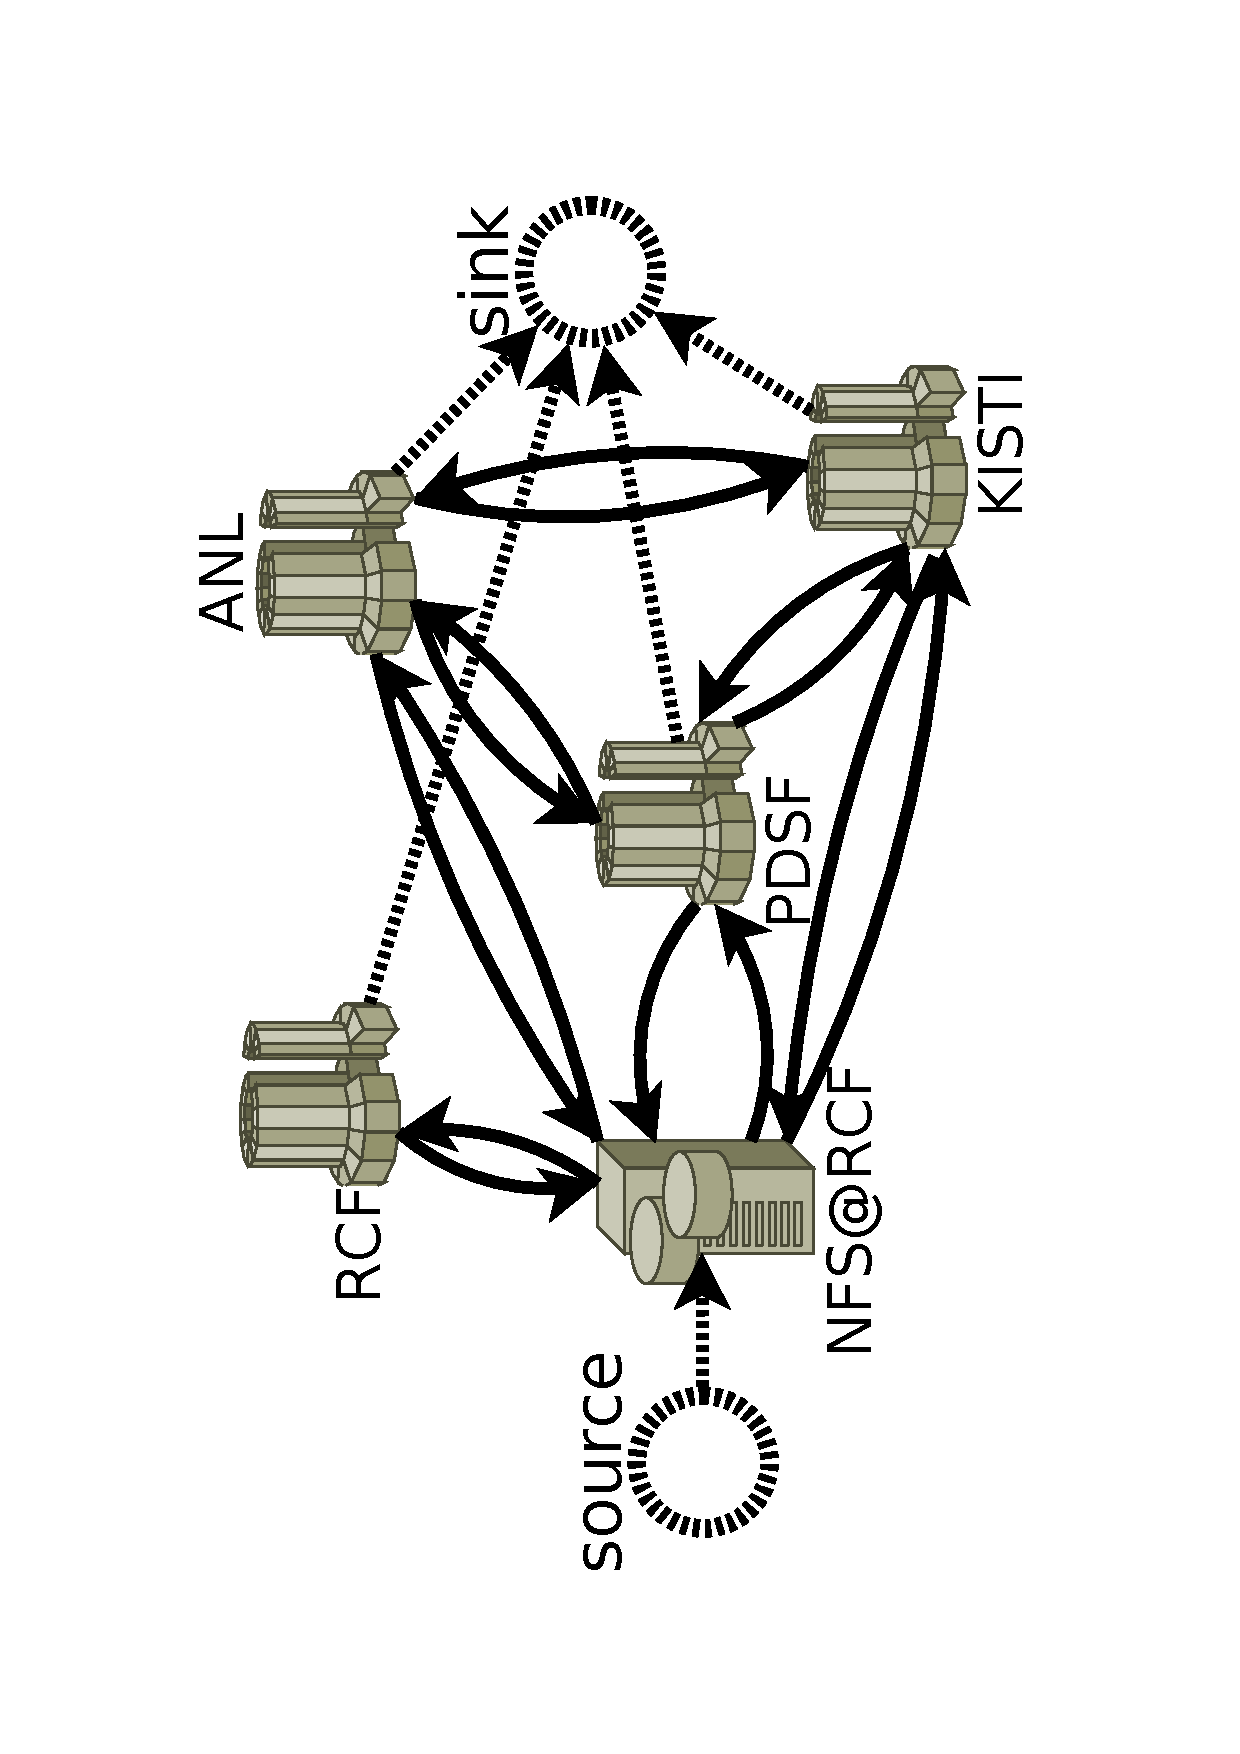
\includegraphics [trim= 30mm 30mm 30mm 30mm , clip, angle =-90, width=0.7\textwidth]{pic/real_network.pdf}
	\end{center}
	\label{real_network}
\end{figure} 
\vspace{-3mm}
Output flow problem can be formulated similarly.
\end{frame}

\begin{frame}\frametitle{Solving procedure}
\begin{block}{}
Problems for input and output transfers can be solved independently under assumptions: 
\begin{itemize}
\item Full-duplex links,
\item In a steady state at each node $Processed\_input\_data= \beta \cdot created\_output\_data$, where~$\beta = const.\leq 1$.
\end{itemize}
\end{block} 

\begin{block}{Solving procedure}
\begin{enumerate}
\item Calculate capacities of dummy edges using monitoring data.
\item Solve the problem for output data flows.
\item Recalculate remaining network capacity.
\item Solve the problem for input transfers.
\end{enumerate}
\end{block}    
\end{frame}


\begin{frame}\frametitle{Plan execution}

\begin{columns}[c] % the "c" option specifies center vertical alignment
    \column{.6\textwidth} % column designated by a command 	

\begin{block}{}
\begin{itemize}
\item A local handler at each node receives the plan:

\begin{itemize}
\footnotesize
\item Flows of outgoing edges - how much data of each type should be send over that link.
\item Flow of dummy edges - how much data should be processed at this node.
 \end{itemize}

\item When a new file arrives, the handler decides according to the plan and current state:

\begin{itemize}
\footnotesize
 \item Process the file (transfer over dummy edge)
 \item OR forward it over one of the links  
 \end{itemize}
 \item Decrease remaining flow of the link by the size of the file after transfer.
\end{itemize}
\end{block}    


\column{.4\textwidth}
\begin{figure}[h]
		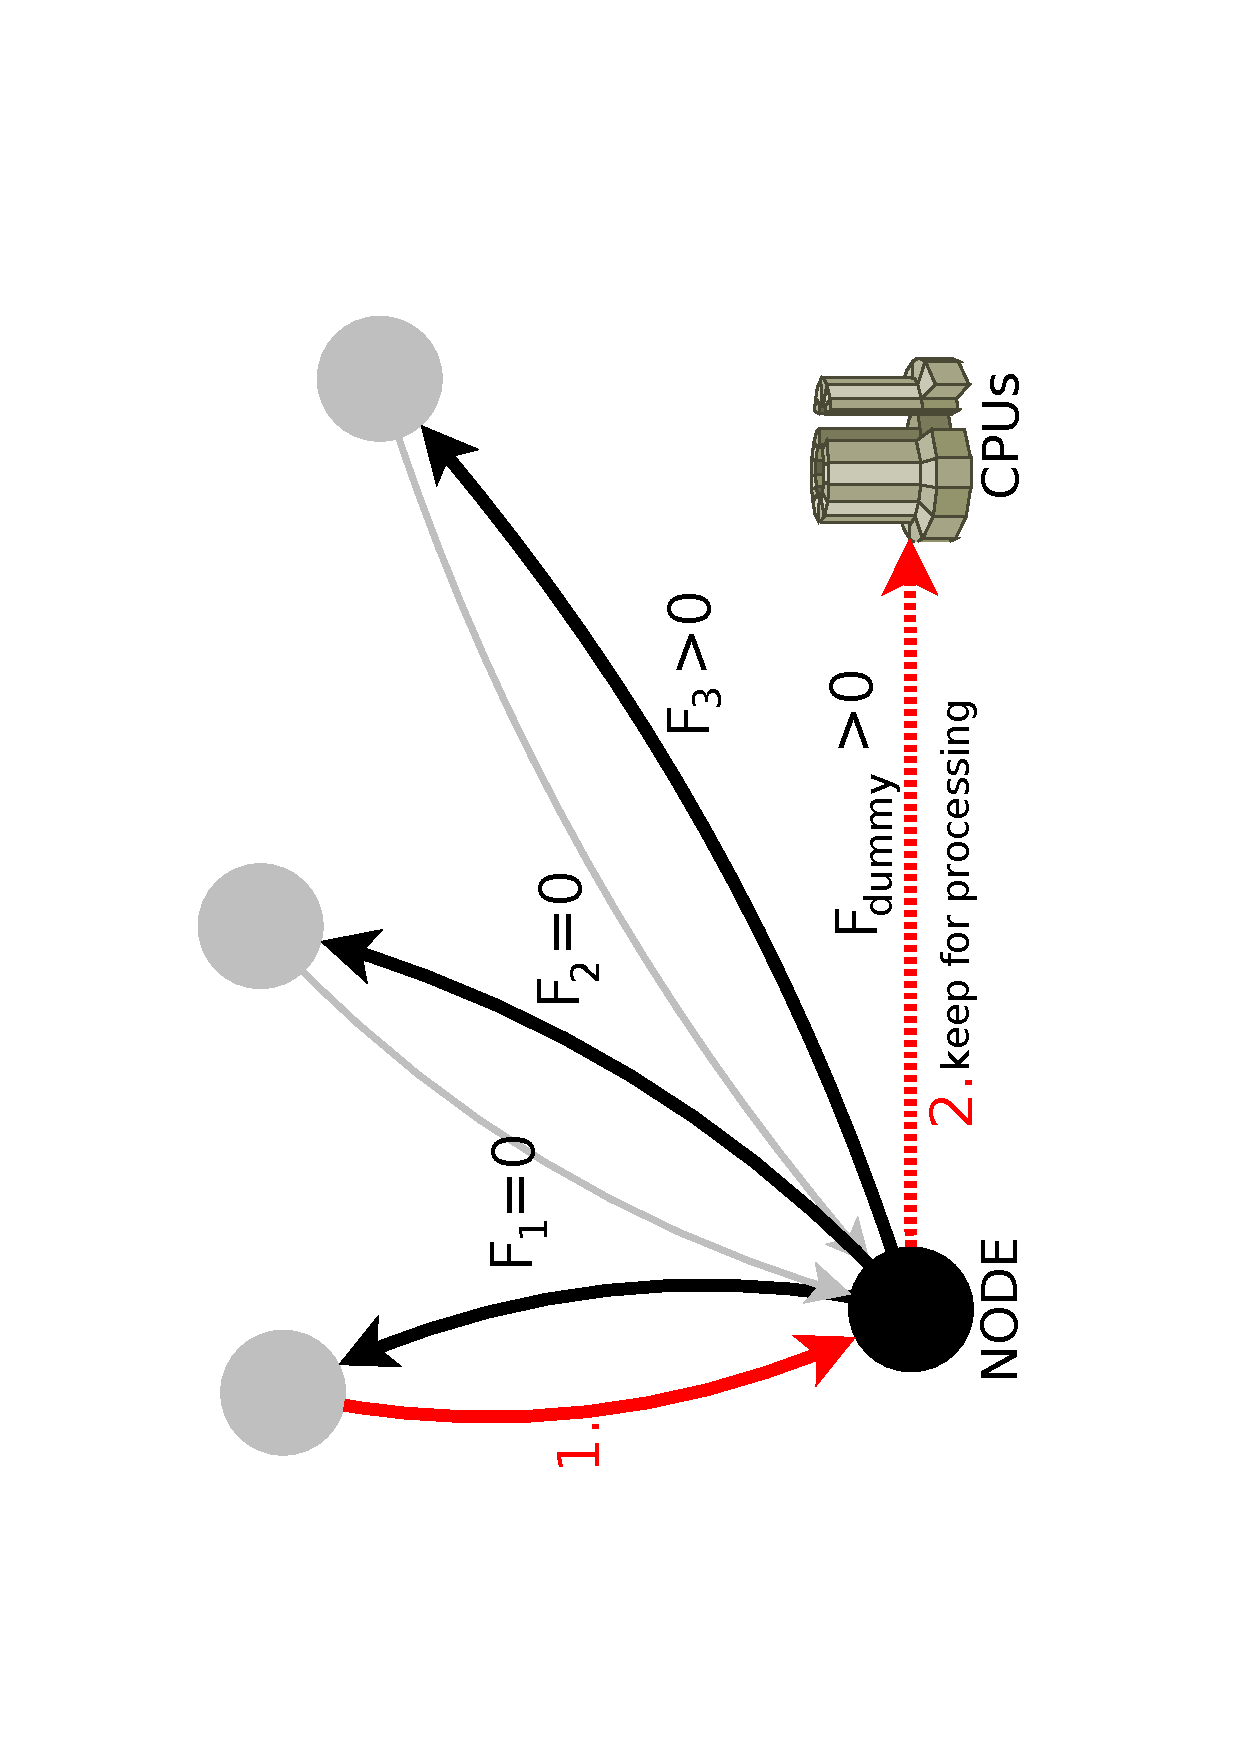
\includegraphics [trim= 30mm 30mm 30mm 30mm , clip, angle =-90, width=\textwidth]{pic/handler_process.pdf}
	\label{real_network}
\end{figure} 

\begin{figure}[h]
		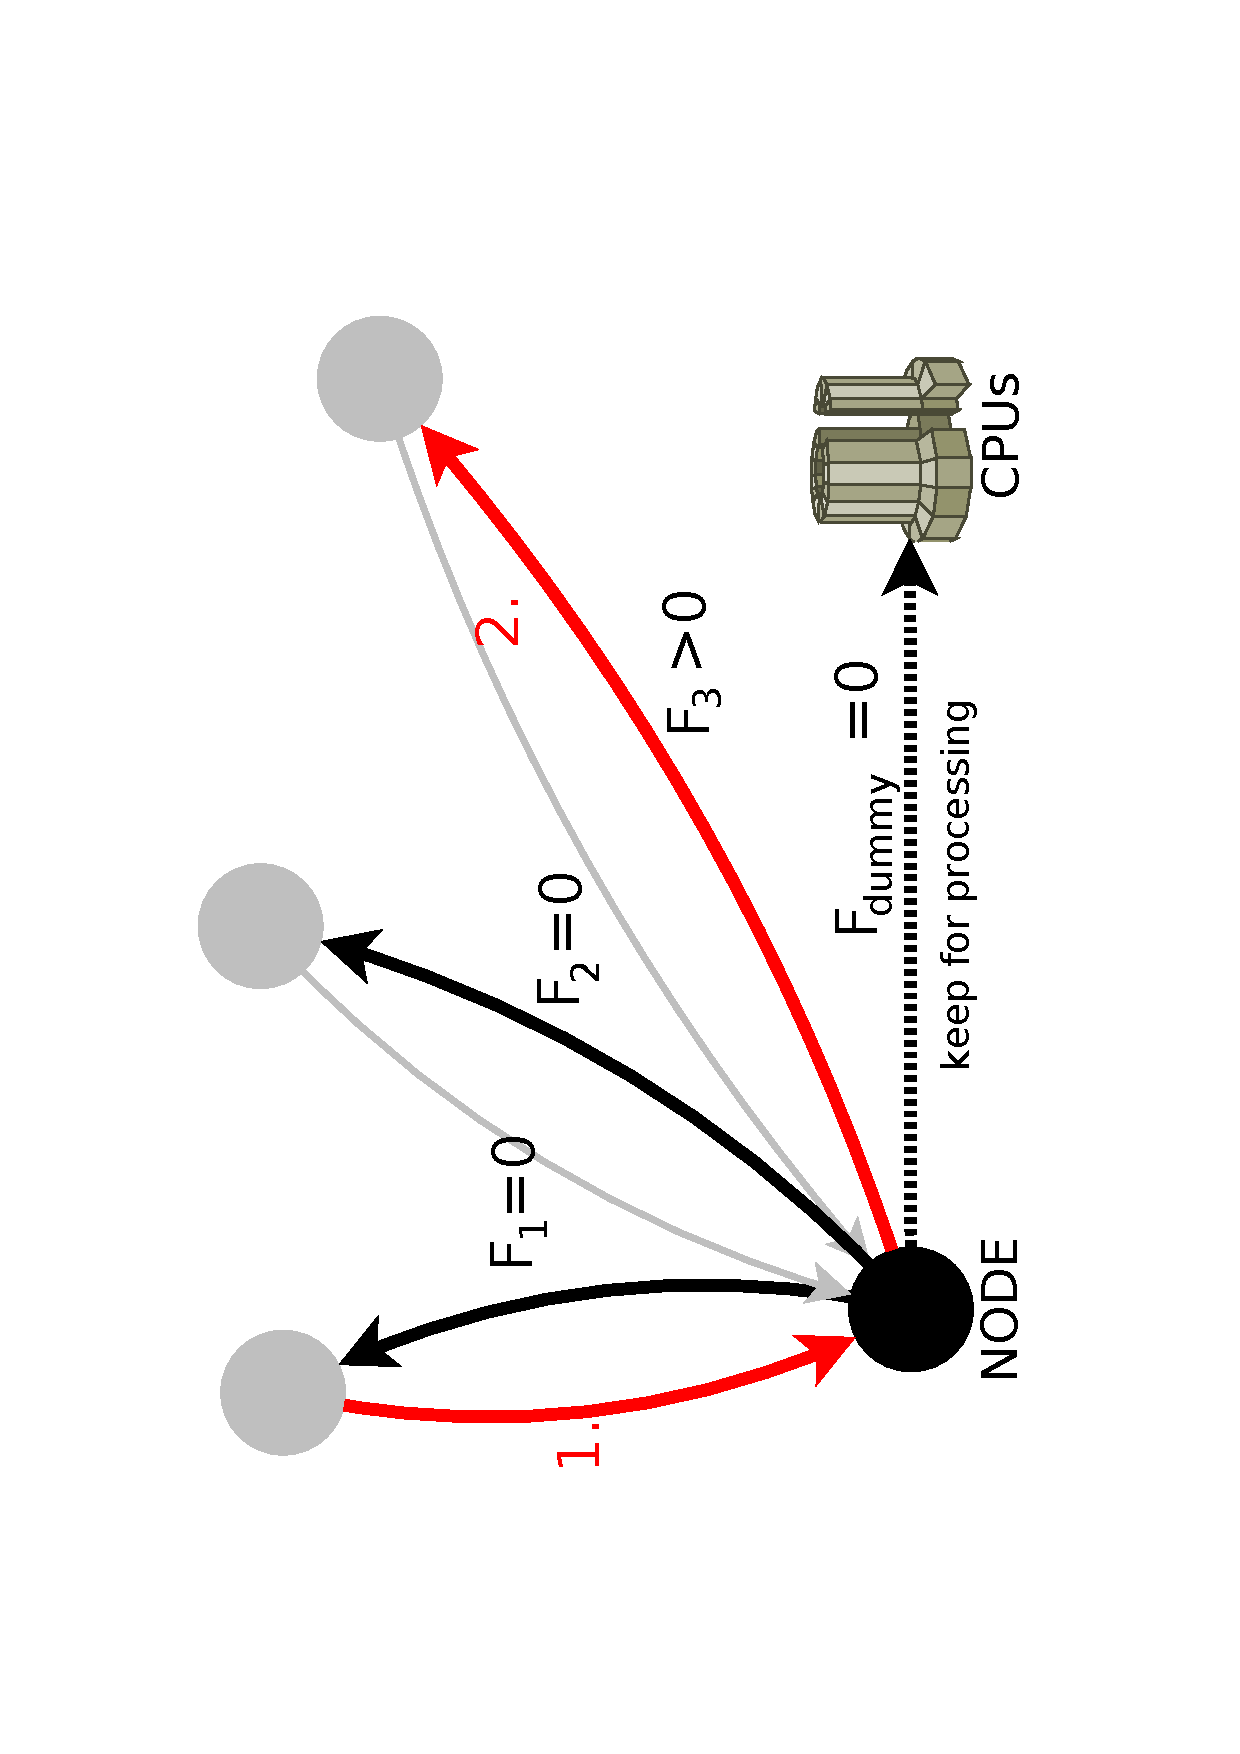
\includegraphics [trim= 30mm 30mm 30mm 30mm , clip, angle =-90, width=\textwidth]{pic/handler_forwarddia.pdf}
	\label{real_network}
\end{figure} 
\end{columns}

\end{frame}

\begin{frame}\frametitle{Network flow model: summary}
\begin{small}
\begin{block}{}
\begin{itemize}
\item This procedure is expected to compute feasible data transfers such that
CPUs in Grid are busy with computational jobs while not exceeding local disk capacities.
\item The model can provide scalability and adaptability to changing environment.
\item A planer using the model has been implemented and tested.
\item Simulations using real log data of the STAR experiment are being implemented using GridSim (modeling tool widely used in Grid community).   
\item Extend the model to meet the broader scope of requirements: several data sources, real network topology, heterogeneous resources and load.  
\item Improve the planner performance in order to enable online scheduling in real environment. 
\item Deploy to data production system of the Star experiment. Test and collect statistics.
\end{itemize}
\end{block}
\end{small}
\end{frame}


\section{Conclusion}

\begin{frame}\frametitle{Conclusion}
\begin{block}{}
\begin{itemize}
\item Automated and scalable planning and optimization of distributed computations are highly required in data intensive computational fields such as High Energy and Nuclear Physics. Resent works has revealed the potential of global planning for this task.
\item A CSP for scheduling of data production in Grid was formulated. 
\item The simulations based on log data has shown that the proposed approach systematically provides a smaller makespan and adapts to the increase of transfer overheads better then the other simulated  heuristics.
\item Network flow model has been developed to address the limitations of CP model. Its further development and testing is ongoing.
\item Performance of a wide scope of caching algorithms was simulated using access patterns derived from log files of HENP experiments. The most appropriate ones were selected for data managemend in HENP computations. 
\end{itemize}
\end{block}
\end{frame}

\section{Aims of the PhD research}
\begin{frame}\frametitle{Aims of the PhD research}
\begin{footnotesize}
to develop and implement a general methodology for \textbf{planning of data intense computations in a distributed environment} with primary focus on \textbf{data production} in HENP. 
\begin{block}{Goals}
\begin{itemize}
\item \textbf{Mathematical model.} General mathematical model for data production planning. Suitable level of abstraction, extensible. 
\item \textbf{Scalable planer:} Petabytes of data, hundreds of computational sites, real-time planning.
\item \textbf{Adaptability to dynamic changes:} Background network traffic, cluster load by other tasks, downtime, errors, failures.
\item \textbf{Extended versions of the problem.} Several data sources, real network topology, several experiments (users), user analysis case, resource heterogeneity. 
\item \textbf{Evaluation using real log data.} STAR data production, other HENP experiments, scalability tests. 
\item \textbf{Deployment.} Integration into distributed RMS. Deployment to the data production system of the STAR experiment. Testing, statistics collection. 
\end{itemize}

\end{block}
\end{footnotesize}
\end{frame}

\begin{frame}<beamer>[noframenumbering]\frametitle{Publications }
\begin{figure}
	\begin{center}
		\centering
		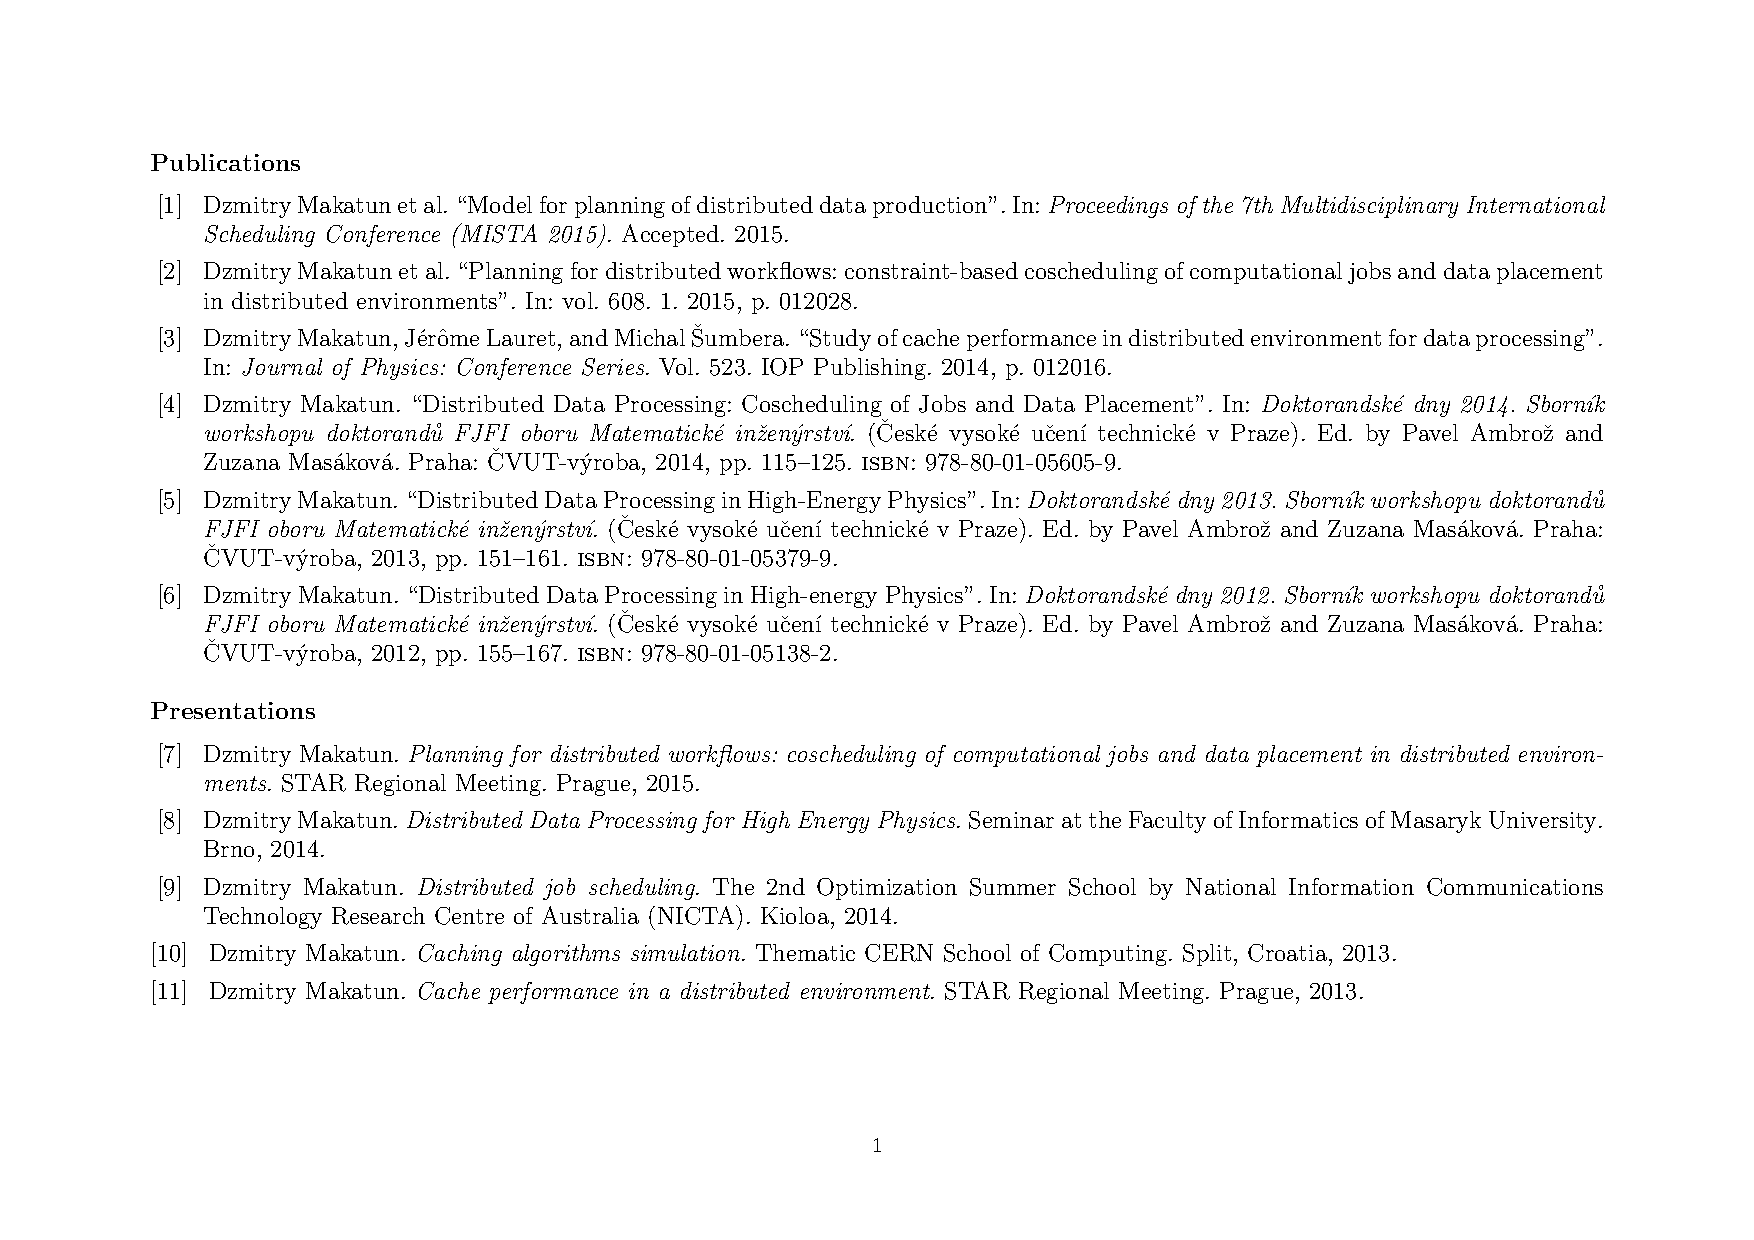
\includegraphics[trim = 20mm 20mm 20mm 20mm,clip,width=\textwidth]{myref.pdf}
	\end{center}
\end{figure}	
\end{frame}

\begin{tiny}
\renewcommand*{\bibfont}{\tiny}
\printbibliography[notkeyword=my]
\end{tiny}


\end{document}
